\documentclass{article}

\usepackage[final]{nips_2017}

% to compile a camera-ready version, add the [final] option, e.g.:
% \usepackage[final]{nips_2017}

\usepackage[utf8]{inputenc} % allow utf-8 input
\usepackage[T1]{fontenc}    % use 8-bit T1 fonts
\usepackage{hyperref}       % hyperlinks
\usepackage{url}            % simple URL typesetting
\usepackage{booktabs}       % professional-quality tables
\usepackage{amsfonts}       % blackboard math symbols
\usepackage{nicefrac}       % compact symbols for 1/2, etc.
\usepackage{microtype}      % microtypography
\usepackage{graphicx}		% to allow images

\graphicspath{ {images/} }

\title{Detecting Motion Blur in Images}

\author{
  Karan Varindani \\
  \And
  Wenyang Zhang \\
  \And
  Sibo Zhu \\
}

\begin{document}

\maketitle

\begin{abstract}
  Our project aims to estimate motion blur from a single, blurry image. 
  We propose a deep learning approach to predict the probabilistic distribution 
  of motion blur at the patch level using a Convolutional Neural Network (CNN).
\end{abstract}

\section{Our approach}
We approached the problem by slicing 100 images into 30x30 patches, and applied
our own motion blur algorithm to them (with a random rate of 50\%). We then labeled 
the blurry and non-blurry patches with 0s and 1s (0 for still, 1 for blurry), and
loaded the modified images in as our training data.
  
\subsection{Generating the training data}
We generated the training data using images from the 
\textit{\href{http://host.robots.ox.ac.uk/pascal/VOC/voc2010/}{Pascal Visual Object 
Classes Challenge 2010 (VOC2010)}} data set. Our work was done in Python using the 
\textit{PIL}, \textit{numpy}, \textit{opency}, and \textit{os} libraries.

Once we had the original images from \textit{Pascal}, we had to modify them to fit our 
needs. We needed to have 100 images, each partially blurred and with a corresponding 
matrix indicating which part of the image is blurred. 

We achieved this by:
\begin{enumerate}
  \item Making a blurred copy of the original image. 
  \item Cutting both images (original and blurry) into $30\times30$ patches.
  \item Creating a 2D List in Python of size $30\times30$, to represent each image patch
  We initialize each element to 0 (to represent non-blurry). 
  \item Picking half the patches from the list and marking them as 1 (to represent 
  blurry).
  \item Putting the final image together to get a partially-blurred, qualifying image 
  (and its corresponding matrix).
  \item Saving the image as "n.jpg" (where n is the serial number of the image), and 
  adding the matrix to a list (to form a 3D 'list of lists') containing the matrices 
  of all the image.
\end{enumerate}

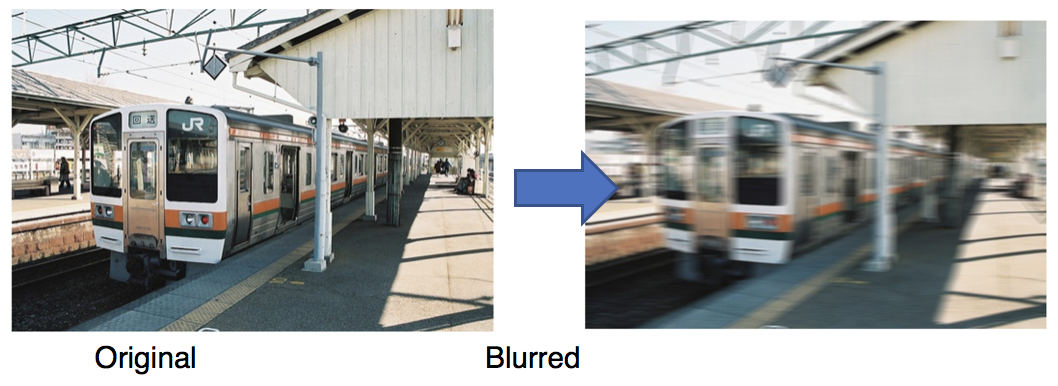
\includegraphics[width=\textwidth]{blur} \\
\textit{Image of the original-to-blur process.} \\ 
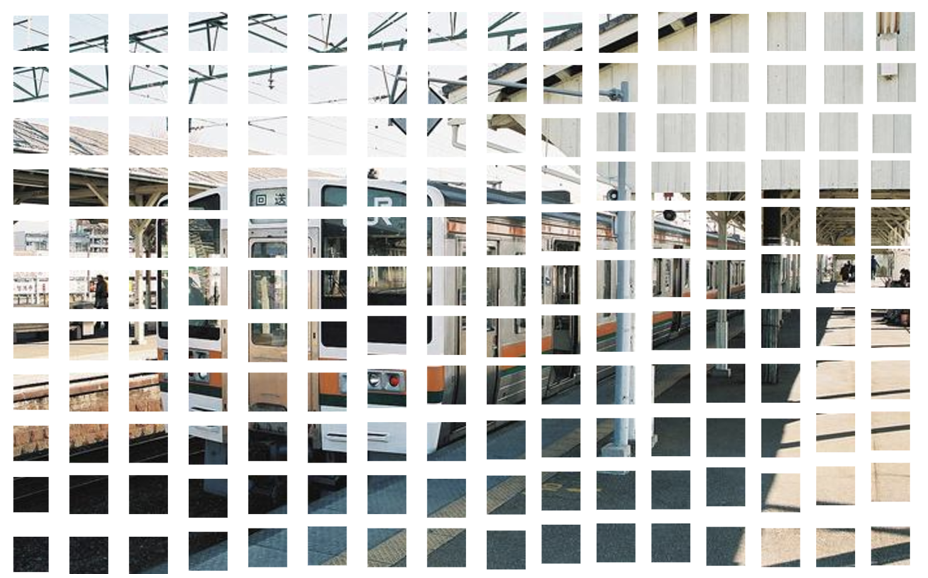
\includegraphics[width=\textwidth]{patches} \\
\textit{Image of the image splitting process.} \\
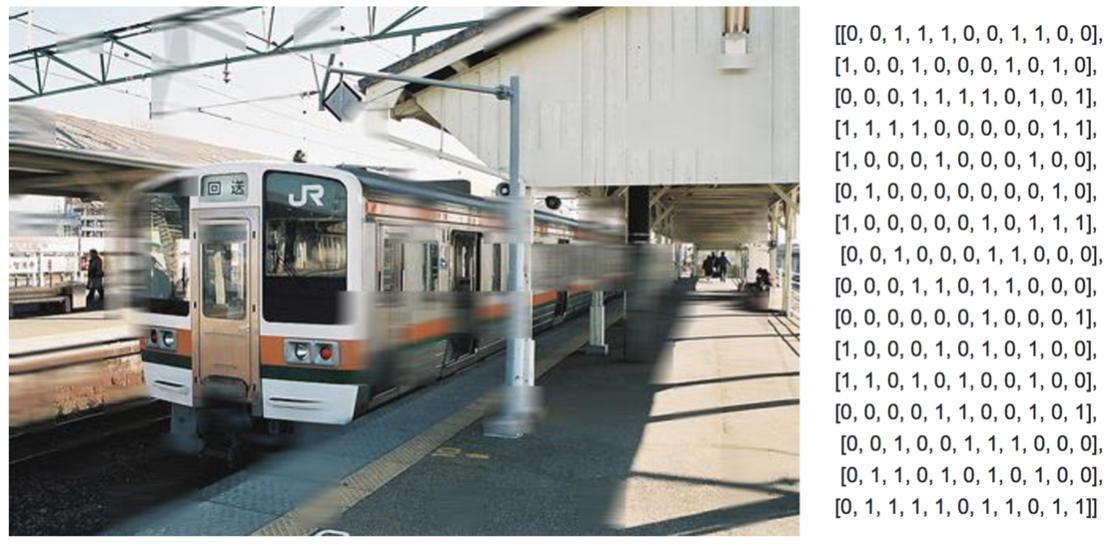
\includegraphics[width=\textwidth]{matrix} \\
\textit{The final image with its corresponding matrix.} \\

We repeat the above for all 100 images, until we end up with a folder containing 
partially-blurred images \textit{"0.jpg"} through \textit{"100.jpg"}, and a 3D list 
(named \textit{"labels"}) that contains 100 matrices. This lets us access the matrix for 
image \textit{"31.jpg"}, for example, by querying for \textit{"labels[31]"}.

\section{Learning the Convolutional Neural Network (CNN)}
Once we had the prepared images, \textbf{we loaded them into our training set.} We ran 
into a problem loading the images into a \textit{numpy} array, where our images were of 
the form (30,30,3), while the \textit{Keras.Conv2D} layer required input to be of the form 
(3,30,30). We solved this by using the \textit{numpy.swapexes()} function to alter the 
images' shape in order to fit the convolutional layer.

\paragraph{We then apply the CNN learning model.}
First, we apply a Convolution2D layer with $7\times7$ filters, followed by a \textit{ReLU} 
function. The \textit{Conv} layer's parameters consiste of a set of learnable filters. 
Each filter is small spatially, but extends through the depth of the input volume. 

\paragraph{During the forward pass,} 
we slide each filter across the width and height of the input 
volume and compute the dot products between the entries of the filter and the input at 
any position. \textit{ReLU} is the rectifier function- an activation function that can be 
used by neurons, just like any other activation function. A node using the rectifier 
activation function is called a \textit{ReLU node}. \textit{ReLU} sets all negative values 
in the matrix x to 0, and all other values are kept constant. ReLU us computed after the 
convolution, and thus a nonlinear activation function (like \textit{tanh} or 
\textit{sigmoid}).

After that, \textbf{we add a \textit{MaxPooling2D} layer} with a pool size of $2\times2$. 
MaxPooling is a sample-based discretization process. The objective is to down-sample an 
input representation, reducing its dimensionality and allowing for assumptions to be made 
about features contained in the binned sub-regions. 

We then \textbf{add a \textit{Dropout} layer} with dropout rate of 0.2, which makes our 
learning process faster. Dropout randomly ignoring nodes is useful in CNN models because 
it prevents interdependencies from emerging between nodes. This allows the network to learn 
more and form a more robust relationship. We then do the \textit{'Conv2D, ReLU, 
MaxPooling2D, Dropout'} circle again. Finally, we add a fully-connected layer with 
\textit{ReLU}, and then \textit{softmax} the result. \textit{Softmax} is a classifier at 
the end of the neural network — a logistic regression to regularize outputs to a value 
between 0 and 1. 

\paragraph{We set our model's learning rate to be $0.01$.} This might generally be too 
big, but we made this decision for the sake of brevity - it was the fastest way to show 
a result. We chose a batch size of 126 (because we had large training data). We also 
chose \textit{Adam} as our optimizer as it's the most efficient optimizer for our model.

After training with 100 epochs, \textbf{we had testing accuracy of 92\%}, which is a 
very optimal rate for our model. Our training model is saved in an HDF5 file, 
\textit{"motionblur.h5"}.  

\section*{Acknowledgement}
This report has been prepared for the Boston University Machine Learning course (CS 542), 
taken over the Summer 2, 2017 semester by the listed authors. It is intended to be used 
in compliance of the requirements of the course. 

\section*{References}
\medskip
\small

[1] Jian Sun, Wenfei Cao, Zongben Xu, Jean Ponce. Learning a convolutional neural network 
for non-uniform motion blur removal. CVPR 2015 - IEEE Conference on Computer Vision and 
Pattern Recognition 2015, Jun 2015, Boston, United States. IEEE, 2015, .

[2] “Visual Object Classes Challenge 2010 (VOC2010).” The PASCAL Visual Object Classes 
Challenge 2010 (VOC2010), PASCAL, 2010, host.robots.ox.ac.uk/pascal/VOC/voc2010/.

\end{document}
